\documentclass[11pt]{scrartcl}
%\documentclass[12pt, a4paper]{article}

\newif\ifpdf
\ifx\pdfoutput\undefined
\pdffalse % we are not running PDFLaTeX
\else
\pdfoutput=1 % we are running PDFLaTeX
\pdftrue
\fi

\ifpdf
\usepackage[pdftex]{graphicx}
\else
\usepackage{graphicx}
\fi

\usepackage[utf8]{inputenc}
\usepackage[english]{babel}
%\usepackage{german}
%\usepackage{longtable}
%\usepackage{tocbibind}
%\usepackage{makeidx}
\usepackage[pdftex,pageanchor,colorlinks,pdfborder=0,breaklinks,urlcolor=blue]{hyperref}
\usepackage{amsmath}
\usepackage{amsfonts}
\usepackage{amssymb}
%\usepackage{pdfsync}  % enable tex source and pdf output syncronicity
%\usepackage[all]{xy}
\usepackage{multicol}
%\usepackage{rotating}
%\usepackage{wrapfig}
%\usepackage{subfigure}
%\usepackage{listings}
\usepackage[pdftex,rightbars,color]{changebar}

\usepackage{geometry} % to change the page dimensions
\geometry{a4paper}
\geometry{textwidth=16.5cm,textheight=24.5cm}
\geometry{left=2.5cm,twoside}
\parskip=0 cm
\parindent=0.0cm

\usepackage{fancyhdr} % This should be set AFTER setting up the page geometry
\pagestyle{fancy} % options: empty , plain , fancy

\renewcommand{\labelitemi}{-}

% Tiefe des Inhaltsverzeichnisses
\setcounter{secnumdepth}{2}
\setcounter{tocdepth}{2}

\hypersetup{
    pdftitle={Master Thesis: Tool support for user testing of stereoscopic fatigue},
%    pdfsubject={Subject of the document}, % Subject 
    pdfauthor={Gerhard Roethlin},              % Author
    pdfkeywords={master, fatigue testing software, job description},       % Keywords
}

\title{Master Thesis: Tool support for user testing of stereoscopic fatigue\\
{\large Implementing a flexible and extensible testing framework}}
\author{\normalsize Gerhard R\"othlin 
{\tt  \href{mailto:gerhardr@student.ethz.ch}{gerhardr@student.ethz.ch}}}
\date{}

\ifpdf
\DeclareGraphicsExtensions{.pdf, .jpg, .tif}
\else
\DeclareGraphicsExtensions{.eps, .jpg}
\fi

\begin{document}

\maketitle
%\tableofcontents

\begin{center}
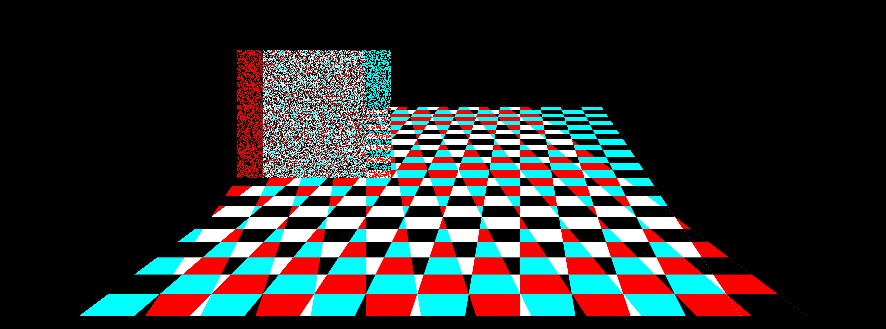
\includegraphics[width=15cm,clip,trim=0cm 0cm 0cm 0cm]{media/title.png}
\end{center}

%\begin{abstract}
%\end{abstract}

\begin{multicols}{2}

%\tableofcontents

\section{Research question}
\paragraph{}
Viewing stereoscopic movies or images is unnatural. The focus and vergence of the eyes have to be decoupled. This strains the eyes, and can lead to fatigue, which makes the consumption of stereoscopic information over longer periods of times hard. But what are the physiological and psychological limits of stereoscopic viewing fatigue? And how can stereo images be composed to reduce fatigue?

Topic of this thesis is to write a Tool that enables exploration of those and similar other questions by providing a flexible and extensible framework for user testing. It is currently unclear how fatigue can be measured properly, and what scenes can be used to specifically test fatigue. Finding out which methods work and which do not is also part of this thesis.

\section{Current Plan}
\paragraph{}
To answer questions on fatigue, experiments with users are conducted. The first experiment is planned to show how much the viewing of stereoscopic information tires the eyes and if adding continuous depth has any influence on this.

Fatigue when viewing stereoscopic pictures is tested by showing images without continuous depth, with free standing objects, and scenes with continuous depth, embedded in a scene.

In both test cases, the time it takes the test subjects to change vergence from one object to an other object is measured. The expectation is that with continuous depth, the adaption to different perceived depths is faster and the slowdown due to fatigue is smaller. The experiments will show if this is valid.

\section{Example requirement}
\paragraph{}
The testing tool should automate steps needed to test 3D related fatigue. A typical test could work as following:

\begin{enumerate}
\item Encode information at a certain perceived stereoscopic depth, so that it can only be extracted when focusing with both eyes. Measure the time it takes the test subject to adapt to this depth and extract the information.
\item Remove the information and place it at an other depth location, measuring reaction time.
\item Repeat step 1 and 2 at a different depth locations.
\item Repeat step 1 and 2 with the information being embedded in a scene that provides a continuous depth clue.
\item Measure response time over a longer period of time, over several test repetitions, with several test subjects.
\item Correlate fatigue based on response time.
\end{enumerate}

\section{Challenges}
\paragraph{}
To perform those tests, a flexible and extensible tool is needed. Some of the requirements that have to be satisfied include:

\begin{enumerate}
\item Supporting stereogram encoding of information. Stereograms are used to confirm that the test subject can fuse a picture at a given location with a given separation.
\item Supporting of various scenes/depth clues
\item Flexible and powerful log format, that can be transformed to be analyzed by established software.
\item User input while looking at screen, such as blind typing and audio feedback.
\item Must support various scenes and scenes changing in various ways, such as camera and object movement.
\end{enumerate}

\section{Baseline features}
\paragraph{}
The software should be created for specific tests, and then later extended to other areas. During development a pilot study will be conducted. Having immediate feedback will help to guide development.

The tool should have at least these baseline featuers:

\begin{itemize}
\item Rendering in 3D
\item Import of 3D models and other data from other applications
\item Rendering of depth maps in random-dot stereograms.
\item Interactive modifications of scene in limited ways during the test
\item Must support anaglyph and dual screen/mirrored viewfinder output
\item Support of basic scene objects, individually enabled
\item Scripting of tests, with randomized parameters
\item Individual control of depth cues, such as relative size, occlusion or stereoscopic seperation
\item Support various input mechanisms such as keyboard, mouse.
\item Record all events
\item Support export of logs in various formats
\end{itemize}

\section{Shopping list}
\paragraph{}
Thoughts about the design:

\begin{itemize}
\item It should be cross platform, so that it works on Mac OS X, Windows and Linux.
\item It should support 3D rendering with HW acceleration, so OpenGL is the way to go
\item QT could serve as GUI/Backend toolkit. It is cross platform and licensed under GPL v2.
\item OpenMesh can be used as mesh loader and storage library. It is licensed under the GPL v2.
\item LUA or some other scripting language can be used to do the interactive stuff. It leaves a lot of freedom to the designer of the scene/test, since most of the functionality would run in script code. LUA is licensed under an MIT style attribution license, which allows use everywhere.
\item Test files would contain media (pictures, models, textures), lua code (for building scenes out of the media, and animating, moving, randomizing) and a master file that binds it together.
\item Templates or a test builder application will be built to create those lua scripts in standard cases, but writing code would give {\textit a lot} of flexibility to the test designer.
\end{itemize}

\section{Evaluation}
\paragraph{}
A first pilot study without the use of the finished tool is conducted to evaluate if the test methodology is valid. This will also decide which data is logged in what way, and how it can be evaluated.

The current proposition is that user input consists of key presses. Reaction time of switching between different perceived depth locations is logged in a time stamp format. An optional post processor can aggregate this data, and transform it in various representations. Alternatives include using audio equipment to store recordings of the test, and use volume or voice recognition for quantitative analysises. 

\section{Milestones}
\begin{itemize}
\item 2008.01.07: Start
\item 2008.02.07: First basic framework complete
\item 2008.03.07: Evaluated testing frameworks through pilot study. Improve the system to meet the encountered requirements to support a full scale study. Identify potential stimuli and tasks to extend the framework.
\item 2008.04.02: Deadline Paper about fatigue related to continuous depth.
\item 2008.04.07: Improve data analysis capabilities in framework. Write status report to reflect on the current capabilities of the system in context of conducted tests, state resources utilised, propose future improvements.
\item 2008.05.07: Apply the tool to other experiments, evaluate the requirements in other contexts.
\item 2008.06.07: Finish outline for master thesis.
\item 2008.07.07: Master Thesis completed
\end{itemize}

\end{multicols}

\appendix

\section{Links}
\url{http://graphics.cs.uiuc.edu/svn/wickbert/trunk/OpenMesh/LICENSE}

\url{http://trolltech.com/products/qt/licenses/licensing/opensource}

\url{http://www.lua.org/license.html#5}

\url{http://www.rasterbar.com/products/luabind/docs.html}

\url{http://lua-users.org/wiki/LunaWrapper}

\url{http://en.wikipedia.org/wiki/Random_dot_stereogram}




\end{document}
\end
